\documentclass[10pt,a4paper]{article}
\usepackage[margin=17mm]{geometry}
\usepackage{graphicx}
\usepackage{array}
\usepackage[T1]{fontenc}
\usepackage{lmodern}
\pagestyle{empty}
\setlength{\parindent}{0pt}
\setlength{\parskip}{5pt}
\begin{document}
{\Large\bfseries BINSTD encoded theorem: local full-gate addendum}\\[3pt]
{\small 27 October 2026 UTC \quad Frozen producer \texttt{6409590d} \quad Execution head \texttt{98fca453}}

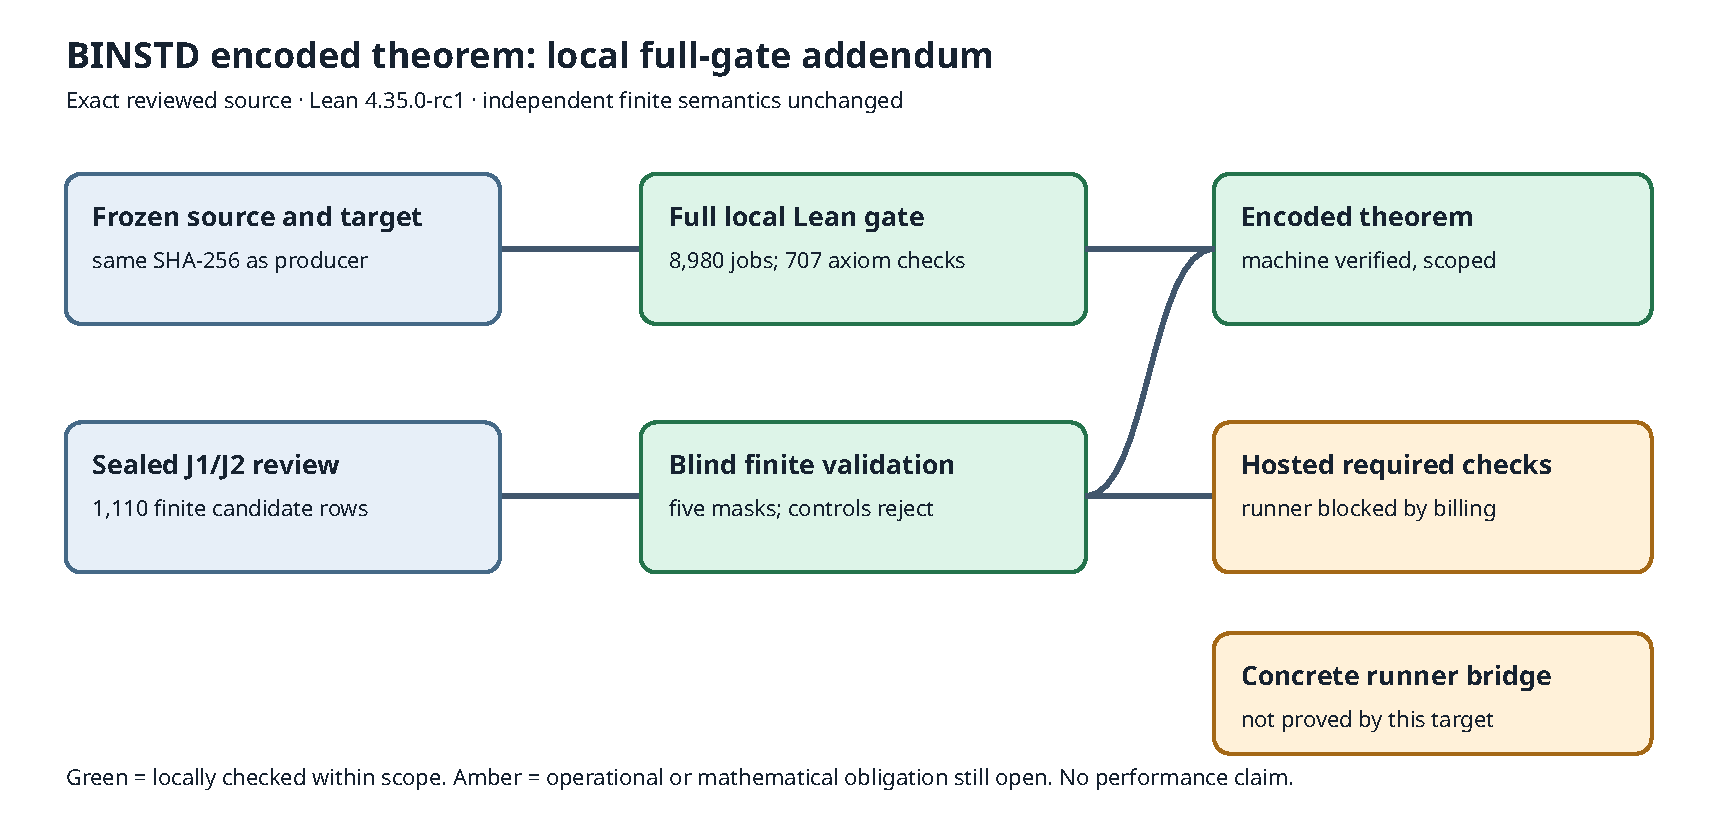
\includegraphics[width=\textwidth]{diagram.pdf}

\textbf{Observation.} The pinned Lean 4.35.0-rc1 root built 8,980 Lake jobs.
The repository's exact formal verifier returned \texttt{machine\_verified}:
the named module built, the project audit found 707 theorem declarations using
only permitted standard axioms, and the requested-theorem audit passed. The
source, target, toolchain and manifest hashes match the independently reviewed
producer inputs. The verifier found no forbidden construct or infrastructure
failure.

\vspace{3pt}
\begin{tabular}{@{}p{0.27\textwidth}p{0.27\textwidth}p{0.40\textwidth}@{}}
\textbf{Review claim} & \textbf{Sealed snapshot} & \textbf{2026-10-27 local update}\\\hline
C1 finite masks/counts & validated scoped & unchanged: 1,110 rows independently retained\\
C2 Lean declaration & direct check only & full exact-target gate passed for identical source\\
C3 direct receipt & validated direct scope & unchanged\\
C4 full workspace & not verified & locally machine verified; hosted job did not start\\
C5 polynomial/runner bridge & open & still open for this encoded theorem\\
\end{tabular}

\vspace{3pt}
\textbf{Boundary.} The theorem checks the specified finite XOR-and-shift
predicate. It does not connect that function to polynomial Euclidean remainder
or the archived runner's Frobenius representation, and it supplies no yield or
attack-cost measurement. Separate PR \#2484 contains unmerged cyclotomic and
abstract finite-field proofs. Current-head GitHub Actions are blocked before
runner assignment by the account payment/spending-limit gate; merge and Pages
publication remain pending.

\vspace{2pt}
\textbf{Evidence.} This write-once addendum cites the sealed J1/J2 packet and
the new SHA-bound full-gate validation receipt in the adjacent BINSTD study.
The original review archive remains unchanged. No official scientific status
transition is made.
\end{document}
